\documentclass[conference]{IEEEtran}
\IEEEoverridecommandlockouts
% The preceding line is only needed to identify funding in the first footnote. If that is unneeded, please comment it out.
\usepackage{cite}
\usepackage{amsmath,amssymb,amsfonts}
\usepackage{algorithmic}
\usepackage{graphicx}
\usepackage{textcomp}
\usepackage{xcolor}
\usepackage{booktabs}
\usepackage{adjustbox}
\usepackage{multicol}
\usepackage{float}
\usepackage{array}

\renewcommand{\arraystretch}{1.2}

\def\BibTeX{{\rm B\kern-.05em{\sc i\kern-.025em b}\kern-.08em
    T\kern-.1667em\lower.7ex\hbox{E}\kern-.125emX}}
\begin{document}

\title{Miniproject 2 - Classification of Textual Data \\
{\small COMP551 - Applied Machine Learning}
}

\author{\IEEEauthorblockN{Ege Odaci}
\IEEEauthorblockA{\textit{McGill University} \\
ege.odaci@mail.mcgill.ca}
\and
\IEEEauthorblockN{Rafael Gomes Braga}
\IEEEauthorblockA{\textit{École de Technologie Supérieure} \\
rafael.gomes-braga.1@ens.etsmtl.ca}
\and
\IEEEauthorblockN{Ramon Figueiredo Pessoa}
\IEEEauthorblockA{\textit{École de Technologie Supérieure} \\
ramon.figueiredo-pessoa.1@ens.etsmtl.ca}
}

\maketitle

\begin{abstract}
   In this mini-project, we studied the application of machine learning algorithms to the task of classifying textual data. We based our study on two well-known datasets named 20 NEWSGROUPS and IMDB REVIEWS which are both comprised of collections of text documents and the respective labels. We performed a multi-class classification on the 20 NEWS GROUPS dataset and both binary and multi-class classification on the IMDB REVIEWS dataset. We used the \texttt{Scikit-Learn} and \texttt{Keras} python packages to implement a pipeline for data loading, feature extraction and selection, model training and validation and hyper-parameter selection, to train 19 different machine learning models and compare their performance. Finally, we present our results provide a detailed discussion about our findings. The best two algorithms obtained 96.69\% accuracy in the 20 NEWSGROUPS dataset (multi-class classification) and 88.36\% accuracy in the IMDB REVIEWS dataset (binary classification). Overall accuracy calculation (90.29\%): (7532 * 0.9669 + 25000 * 0.8836) / (7532 + 25000) = 0.9029.
\end{abstract}


\section{Introduction}
\label{section:introduction}

One of the fundamental problems solved by machine learning is text classification, the task of assigning labels to text based on its content. This task has broad applications such as spam detection, sentiment analysis, and topic detection. It can be divided into:

\begin{itemize}
    \item \textbf{Binary Classification:} When there are two possible labels, for example, spam detection (spam or not spam)
    \item \textbf{Multi-class Classification:} When multiple labels are possible, for example detecting to which topic a specific text is talking about
\end{itemize}

In this project, we studied text classification by comparing the performance of 19 machine learning models on binary and multi-class classification tasks in two well-known datasets. We used the \texttt{Scikit-Learn} python package \cite{scikit-learn} to develop our code, since it has an extensive API for common machine learning tasks, such as data loading, model training, metrics computation, and many others. It also has robust implementations of most of the models we wanted to test. Since we also wanted to test how deep learning performs on our tasks, we used the \texttt{Keras} library \cite{chollet2015keras} to implement two deep learning models. As a result, we found out that they outperform the previous seventeen machine learning models.

The next sections explain in detail our work and the results we obtained. Section \ref{section:related_work} mentions some of the previous work found in the literature, Section \ref{section:datasets} describes the datasets we used, the tasks and the feature extraction process, Section \ref{section:proposed_approach} describes our methodology, Section \ref{section:results} shows the results we obtained and Section \ref{section:discussion} provides a discussion about our findings.

\section{Related Work}
\label{section:related_work}
What we call text classification is the task of classifying a document under an already defined category\cite{jindal2015techniques}. Depending on the document, it can be labeled under one class or more than one class. When the document is labeled under one class, it is called ``single label" text classification and when it is labeled under more than one class, it is then called ``multi-label" text classification\cite{jindal2015techniques}. Right now on the web there is an extraordinary amount of information, so much that for us humans it is impossible to process all that. Automatic text classification plays an important role with its machine learning techniques which automatically builds a classifier by learning the characteristics of the categories from a set of pre-classified documents\cite{sebastiani2002machine}. 


\section{Datasets and Setup}
\label{section:datasets}

\subsection{Datasets}

The 20 NEWSGROUPS data set \cite{20NewsgroupsWebsite} is a collection of approximately 20,000 documents containing texts that were posted in different newsgroups. There are a total of 20 classes representing the newsgroups, some of which are closely related to each other, while others are highly unrelated. The task here is to perform multi-class classification, trying to predict which of the 20 possible classes is associated with each document.

This became such a popular dataset for experiments in machine learning that \texttt{Scikit-Learn} provides a function called \texttt{fetch\_20newsgroups} that automatically downloads this dataset and loads it in different variables. The data already comes sorted in training (60\%) and testing (40\%) sets. In our code we decided to use the \texttt{Scikit-Learn} function and this default data split: training (60\%) and testing (40\%).

The IMDB REVIEWS \cite{largeMovieReviewWebsite} is a dataset intended for binary sentiment classification, first introduced by \cite{maas-EtAl:2011:ACL-HLT2011}. It contains a large number of movie reviews (25,000 for training and 25,000 for testing) collected from the IMDB website, alongside their corresponding star ratings, a number from 1 to 10. They are divided into positive and negative classes based on the value of the star ratings: 1-4 means negative and 7-10 means positive. Even though this dataset is intended for binary classification on the positive and negative classes, we also did multi-class classification on it, trying to predict the actual movie score. In this case, there are 8 possible classes (1-4 and 7-10).

For this dataset, we implemented our own python function to manually load the data. The data comes conveniently split into two folders named \textit{/neg} and \textit{/pos}, for the positive and negative classes. For the binary classification task, we use this folder structure to label the data with the two classes. For the multi-class classification task, we need to parse the contents of the documents to get the star rating for each movie and use that as a label. Within the IMDB directories, reviews are stored in text files named following the convention \textit{id\_rating.txt} where \textit{id} is a unique id and \textit{rating} is the star rating for that review.

\subsection{Feature Extraction}

We used three different \texttt{Scikit-Learn} vectorizers approaches to extract numerical features from the textual data. Their use is to generate a \textit{Bag of Words} from the data. Their details are summarized below:

\begin{itemize}
    \item \textbf{CountVectorizer:} Counts each occurrence of each word in the textual data and produces a sparse Bag of Words representation;
    \item \textbf{HashingVectorizer:} Also counts the number of occurrences of the words but uses a hashing algorithm to convert the words into tokens, thus saving memory and being more efficient;
    \item \textbf{TfIdfVectorizer:} Computes the TF-IDF features of the words, which gives lesser importance to the words that appear more often. 
\end{itemize}

These vectorizers have some options that further modify the feature extraction process. We tried different values for those options and found that the following work better for our tasks:

\begin{itemize}
    \item \texttt{stop words = `english'}: In English, there are some words that appear very often in texts but don't have much meaning by themselves, such as ``are", ``the" and ``or". They are called ``stop words", and this option ignores them
    \item \texttt{strip accents = `unicode'}: removes accents from the words
    \item \texttt{ngram range = (1, 2)}: Only used for the 20 NEWS GROUPS dataset. Depending on the context some words don't mean anything by themselves, but they have meaning when they are together. This option makes so the vectorizer also counts occurrences of two words together.
    \item \texttt{analyser = `word'}: Controls how the \texttt{ngrams} option combines words.
    \item \texttt{binary = True}: Sets all non zero counts to 1.
\end{itemize}

Finally, there is a well known preprocessing action that can be applied in the 20NEWSGROUPS dataset to avoid overfitting, which is to remove the `headers', `footers' and `quotes' sections from the data. We observed the classifiers' performance without removing those sections and noted that in fact, overfitting occurs. Thus, all results reported here have the sections removed.

\subsection{Feature Selection}

For feature selection, we again used \texttt{Scikit-Learn} to compute the chi-squared stats between each feature and class. This allows us to identify and drop the features that are less relevant for classification.

\begin{table}[!b]
  \caption{Classifiers used in the project}
  \label{tab:classifiers}
  \begin{tabular}{| m{2cm} | m{6cm} |}
    
    \hline
    ADABOOST       & It is a meta-estimator that starts fitting a classifier on the original dataset then adds extra copies of the classifier on the same dataset. It adjusts the weights of wrongly classified instances. \\
    \hline
     BERNOULLI NB & Naive Bayes classifier for multivariate Bernoulli models. It is compatible with discrete data and designed for binary, boolean features. \\
    \hline
     COMPLEMENT NB 
     (COMPLMTNB) & The main use is to fix the ``severe assumptions" done by the Multinomial Naive Bayes classifier. It is a perfect fit for imbalanced data sets. \\
    \hline
    DECISION TREE & They are non-parametric supervised learning methods used for classification and regression. The main purpose is to create a model which predicts the value of the target variable by rules inferred from the data features. \\
    \hline
    GRADIENT BOOSTING
    (GRDBOOSTING) & It is a generalization of boosting to arbitrary differentiable loss functions. It is a very effective procedure which can be used for regression and classification. \\
    \hline
    LINEAR SVC & It is a different implementation of Support Vector Classification for the case of a linear kernel. \\
    \hline
    LOGISTIC REGRESSION
    (LR)& It is a linear model for classification rather than regression. It can fit binary, One-vs-Rest, or multinomial logistic regression with optional L1, L2, Elastic Net regularization. \\
    \hline
    MULTINOMIAL NB
    (MULTINB)& It is a Naive Bayes classifier that is suitable for classification with discrete features. It requires integer feature counts. \\
    \hline
    NEAREST CENTROID
    (NRSTCENTROID)& Classes are represented by a centroid, with test samples classified to the class with the nearest centroid. \\
    \hline
    PASSIVE AGGRESSIVE
    (PAGGRESSIVE)& It is used for large scale learning. They don't need a learning rate just like Perceptron. But in contrast to Perceptron, they include a regularization parameter C. \\
    \hline
    PERCEPTRON & It is a simple classification algorithm for large scale learning. It doesn't require a learning rate. It updates models only on mistakes. \\
    \hline
    RANDOM FOREST
    (RNDFOREST)
    & It is a meta estimator which fits the number of decision tree classifiers on various sub-samples of the dataset and uses averaging to improve the predictive accuracy and control overfitting. \\
    \hline
    RIDGE CLASSIFIER & It converts the values into a range between -1 to 1 and treats the problem as a regression task. \\
    \hline
    MAJORITY VOTING CLASSIFIER
    (MJRTVOTING)& It combines different classifiers and uses the bulk vote to predict the labels of the classes.\\
    \hline
    SOFT VOTING CLASSIFIER & It is similar to Majority Voting Classifier. The difference is that soft voting returns class labels as argmax of the sum of predicted probabilities.\\
    \hline
    STACKING CLASSIFIER & 
    It is a method that is used to combine estimators in order to reduce their biases.\\
    \hline
  \end{tabular}
\end{table}

\section{Proposed Approach}
\label{section:proposed_approach}

Initially, we based our implementation on the examples presented in Scikit-Learn \cite{scikit-learn}, however, we greatly restructured the code and added more classifiers and options. We use python's \texttt{argparse} package to allow the user to modify the program behavior by specifying the number of options. It is possible to select which vectorizer will be applied, which classifiers and databases will be used, how the results will be presented, and many other options. All the options are explained in the project's README file and a quick explanation can also be viewed by running the program with the \textbf{-h} option (\textit{python main.py -h}). Based on these options, our final code performs the following pipeline:

\begin{enumerate}
    \item Load the datasets
    \item Use a vectorizer to extract features from the textual data
    \item Select the best features using the chi-squared metric
    \item Train the selected classifiers on the selected databases
    \item Validate the models using k-fold cross validation
    \item Print metrics reports about the performances of the classifiers
    \item Plot the accuracy and training and testing time of each classifier
\end{enumerate}

You can perform grid search and find the best parameters for each classifier using option \textbf{-gs} (\textit{python main.py -gs}). Those best parameters are stored as JSON files inside the \textit{model selection} folder. They will be used the next time the main program runs.

We used a total of 19 classifiers in our project. Five of them are the ones proposed in the assignment's instructions while fourteen are other classifiers that we decided to try. Table \ref{tab:classifiers} presents a brief description of seventeen of them that are taken from the \texttt{Scikit-Learn} documentation website \footnote{https://scikit-learn.org/0.19/index.html} \footnote{Our MAJORITY VOTING CLASSIFIER implementation combined COMPLEMENT NB, RIDGE CLASSIFIER, LINEAR SVC, LOGISTIC REGRESSION, PASSIVE AGGRESSIVE CLASSIFIER, and RANDOM FOREST CLASSIFIER.} \footnote{Our SOFT VOTING CLASSIFIER implementation combined COMPLEMENT NB, LOGISTIC REGRESSION, MULTINOMIAL NB, and RANDOM FOREST CLASSIFIER.} \footnote{Our STACKING CLASSIFIER implementation used COMPLEMENT NB, RIDGE CLASSIFIER, LINEAR SVC, LOGISTIC REGRESSION, PASSIVE AGGRESSIVE CLASSIFIER, RANDOM FOREST CLASSIFIER, and used the final estimator as LINEAR SVC.}.

Besides seventeen classifiers described in Table \ref{tab:classifiers}, the last two classifiers that we used are the deep learning neural networks implemented with \texttt{Keras}\cite{chollet2015keras}. The architecture is explained below:

\begin{itemize}
    \item \textbf{KERAS DL 1:} Is a simpler network with just one hidden layer, composed by 10 neurons with a ReLU activation function. The output layer uses a sigmoid activation function;
    \item \textbf{KERAS DL 2:} We used the following layers: \textbf{Layer 1}: Embedding (maximum features = 6000, embed size = 128). Embedding turns positive integers (indexes) into dense vectors of fixed size. \textbf{Layer 2}: Bidirectional (LSTM (32, return sequences = True)). Bidirectional wrapper for RNNs. LSTM = Long Short-Term Memory layer. \textbf{Layer 3}: Global Max Pool 1D = Global Max pooling operation for 3D data. \textbf{Layer 4:} Dense (20, activation = ReLU). Just a regular densely-connected NN layer composed by 10 neurons with a ReLU activation function. \textbf{Layer 5:} Dropout (0.05). Applies Dropout to the input. \textbf{Layer 6}: The output layer that uses a sigmoid activation function.
\end{itemize}


\section{Results}
\label{section:results}

Here, we present the results we obtained. Because of space limitations, we only show the most relevant data and findings of our work. Complete descriptions, images, tables, and logs, that were generated by our program, can be accessed in the \textit{results} folder.

\medskip

\begin{table}[H]
\caption{20 NEWS GROUPS Multi-Class Classification with Best parameters.Times are displayed in seconds}
\label{table:20news_best}
\begin{center}
\begin{adjustbox}{max width=0.99\textwidth}
\begin{tabular}{|l|l|l|l|}
\hline
   ML Algorithm                    & Accuracy(\%)  & Train time  & Test time  \\
  \hline
 ADABOOST           & 44.04\%                & 19.26                   & 1.015               \\
 BERNOULLINB                   & 62.56\%                & 0.07593                 & 0.0528              \\
 COMPLMTNB                  & 71.22\%                & 0.0646                  & 0.01039             \\
 DECISIONTREE      & 44.72\%               & 9.037                   & 0.006431            \\
GRDBOOSTING  & 59.43\%                & 658.5                   & 0.3929              \\
KNEIGHBORS        & 8.48\%                 & 0.003191                & 1.298               \\
 LINEARSVC                     & 69.82\%                & 0.8115                  & 0.008989            \\
 LR           & 69.28\%                & 22.88                   & 0.01089             \\
 MULTINB                 & 68.79\%                & 0.07197                 & 0.01174             \\
NRSTCENTROID               & 66.70\%              & 0.01669                 & 0.01906            
\\
PAGGRESSIVE & 69.62\%               & 2.319                   & 0.01587             \\
 PERCEPTRON                      & 53.86\%                & 0.4178                  & 0.0171              \\
RNDFOREST      & 63.71\%                & 7.79                    & 0.3067              \\
RIDGE               & 70.02\%               & 3.12                    & 0.02272             \\
MJRTVOTING    & 70.37\%                & 31.06                   & 0.4181              \\
SOFTVOTING         & 71.73\%                & 28.07                   & 0.3526              \\
STACKING            & 71.28\%                & 184.0                   & 0.368              \\
\hline
\end{tabular}
\end{adjustbox}
\end{center}
\end{table}

\begin{table}[H]
\caption{IMDB using Binary Classification With Best Parameters.Times are displayed in seconds}
\label{table:imdb_bin_best}
\begin{center}
\begin{adjustbox}{max width=0.99\textwidth}
\begin{tabular}{|l|l|l|l|l|l|l|}

\hline
 ML Algorithm                    & Accuracy(\%)  & Train time & Test time \\
 \hline
 ADABOOST          & 84.60\%                & 103.3                   & 5.553               \\
BERNOULLINB                   & 81.28\%                & 0.02759                 & 0.02151             \\
 COMPLMTNB                  & 83.93\%               & 0.01739                 & 0.00831             \\
 DECISIONTREE       & 74.14\%               & 7.808                   & 0.01236             \\
 GRDBOOSTING  & 82.86\%                & 100.8                   & 0.06589             \\
 KNEIGHBORS         & 82.66\%              & 0.006417                & 13.02               \\
 LINEARSVC                     & 87.13\%               & 0.2095                  & 0.004025            \\
 LR            & 87.75\%               & 1.075                   & 0.005046            \\
 MULTINB                 & 83.93\%              & 0.01648                 & 0.0088              \\
 NRSTCENTROID               & 84.65\%               & 0.01818                 & 0.01677             \\
 PAGGRESSIVE & 88.07\%             & 0.8581                  & 0.003922            \\
 PERCEPTRON                      & 80.64\%                & 0.09105                 & 0.007187            \\
RNDFOREST       & 85.45\%               & 8.792                   & 0.7235              \\
 RIDGE                & 86.90\%                & 0.5019                  & 0.00815             \\
 MJRTVOTING     & 87.88\%                & 10.81                   & 0.7945              \\
 SOFTVOTING         & 87.73\%                & 10.29                   & 0.6372              \\
 STACKING             & 88.29\%              & 93.17                   & 0.6377             \\
\hline
\end{tabular}
\end{adjustbox}
\end{center}
\end{table}

\begin{table}[]
\caption{IMDB Multi-Class Classification with Best parameters.Times are displayed in seconds}
\label{table:imdb_multi_best}
\begin{center}
\begin{adjustbox}{max width=0.99\textwidth}
\begin{tabular}{|l|l|l|l|l|l|l|}
\hline
ML Algorithm                    & Accuracy(\%) & Train time  & Test time  \\
\hline
 ADABOOST           & 38.02\%                & 122.9                   & 7.493               \\
BERNOULLINB                   & 37.03\%               & 0.04714                 & 0.04163             \\
 COMPLMTNB                  & 37.34\%               & 0.03856                 & 0.01853             \\
 DECISIONTREE      & 30.82\%               & 7.022                   & 0.01285             \\
 GRDBOOSTING  & 37.88\%                & 875.0                   & 0.5061              \\
KNEIGHBORS        & 37.26\%               & 0.006438                & 14.09               \\
 LINEARSVC                     & 40.80\%                & 0.5486                  & 0.0185              \\
 LR            & 42.04\%                & 9.692                   & 0.01969             \\
 MULTINB                 & 37.82\%               & 0.03519                 & 0.01996 \\
 NRSTCENTROID               & 37.33\%                & 0.02599                 & 0.03267             \\
 PAGGRESSIVE & 41.81\%                & 0.5453                  & 0.0195      \\
 PERCEPTRON                      & 31.60\%              & 0.4152                  & 0.0189              \\
 RNDFOREST      & 37.72\%                & 9.598                   & 0.7072              \\
RIDGE                & 38.55\%                & 2.797                   & 0.0416              \\
MJRTVOTING & 41.46\%
& 17.2                    & 0.9589 
\\
SOFTVOTING        & 40.72\%               & 16.47                   & 0.7836              \\
 STACKING            & 40.99\%                & 110.3                   & 0.8278             \\
\hline
\end{tabular}
\end{adjustbox}
\end{center}
\end{table}

The three tasks we explored are:

\begin{itemize}
    \item Binary classification for the IMDB REVIEWS dataset 
    \item Multi-class classification for the IMDB REVIEWS dataset
    \item Multi-class classification for the 20 NEWS GROUPS dataset
\end{itemize}

For each task, we first ran all algorithms using ``default parameters" (values for the parameters that are commonly used for text classification tasks). Then we performed grid search to get the values for the parameters that give the best performance. We summarize the results with the best parameters in Tables \ref{table:20news_best}, \ref{table:imdb_bin_best} and \ref{table:imdb_multi_best}.

Figures \ref{fig:20news_plot}, \ref{fig:imdb_bin_plot} and \ref{fig:imdb_multi_plot} present plots of the algorithms' accuracy score on the three tasks using the best parameters.

\begin{figure}[H]
\centering
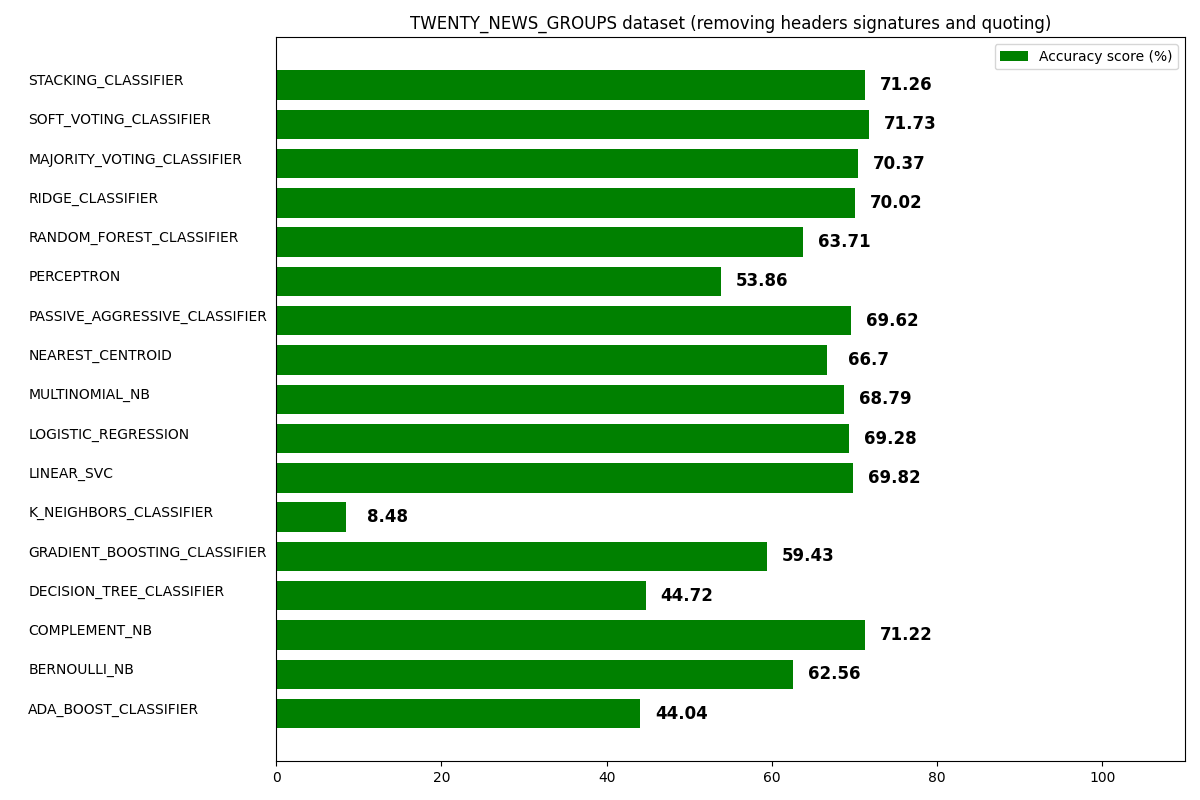
\includegraphics[scale = 0.21]{figs/all_classifiers_20newsgroups_and_imdb_using_binary_classification/TWENTY_NEWS_GROUPS-just_accuracy_score.png}
\caption{Accuracy score of the classifiers in the 20 NEWS GROUPS binary classification task using the best parameters}
\label{fig:20news_plot}
\end{figure}

\begin{figure}[H]
\centering
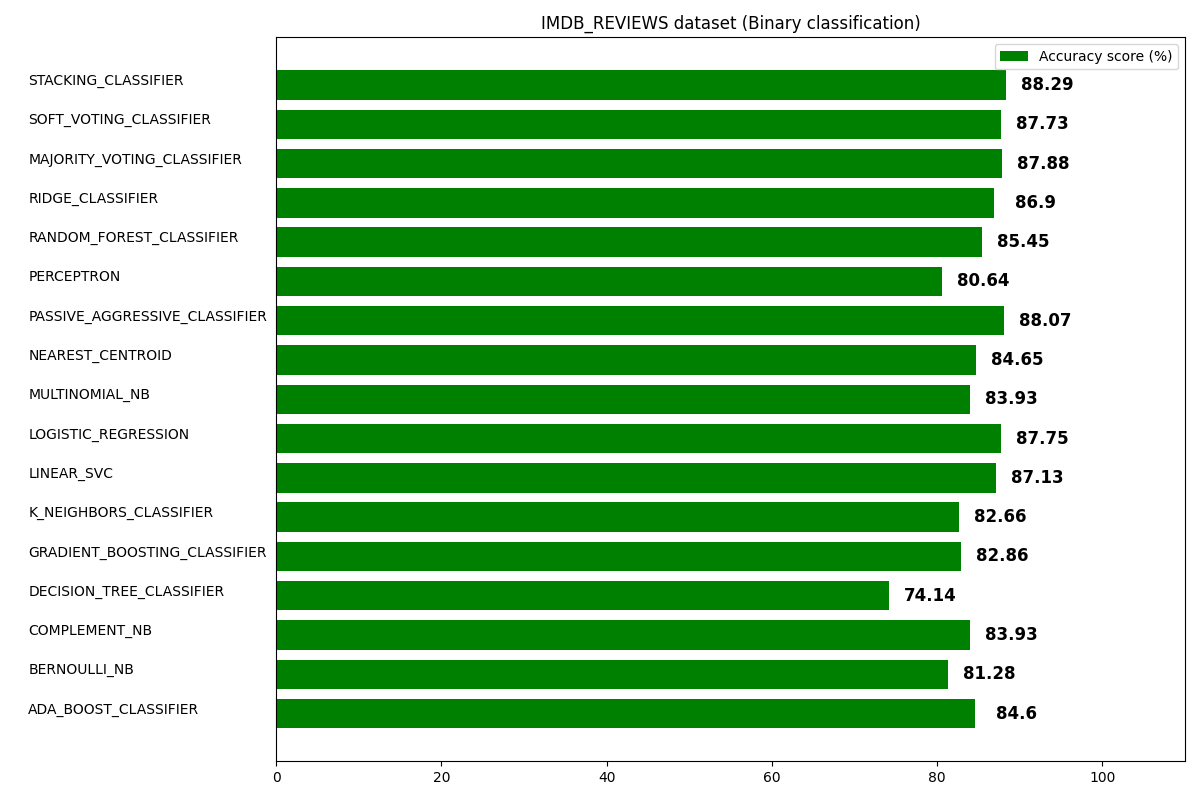
\includegraphics[scale = 0.21]{figs/all_classifiers_20newsgroups_and_imdb_using_binary_classification/IMDB_REVIEWS_binary_classification-just_accuracy_score.png}
\caption{Accuracy score of the classifiers in the IMDB REVIEWS binary classification task using the best parameters}
\label{fig:imdb_bin_plot}
\end{figure}

\begin{figure}[H]
\centering
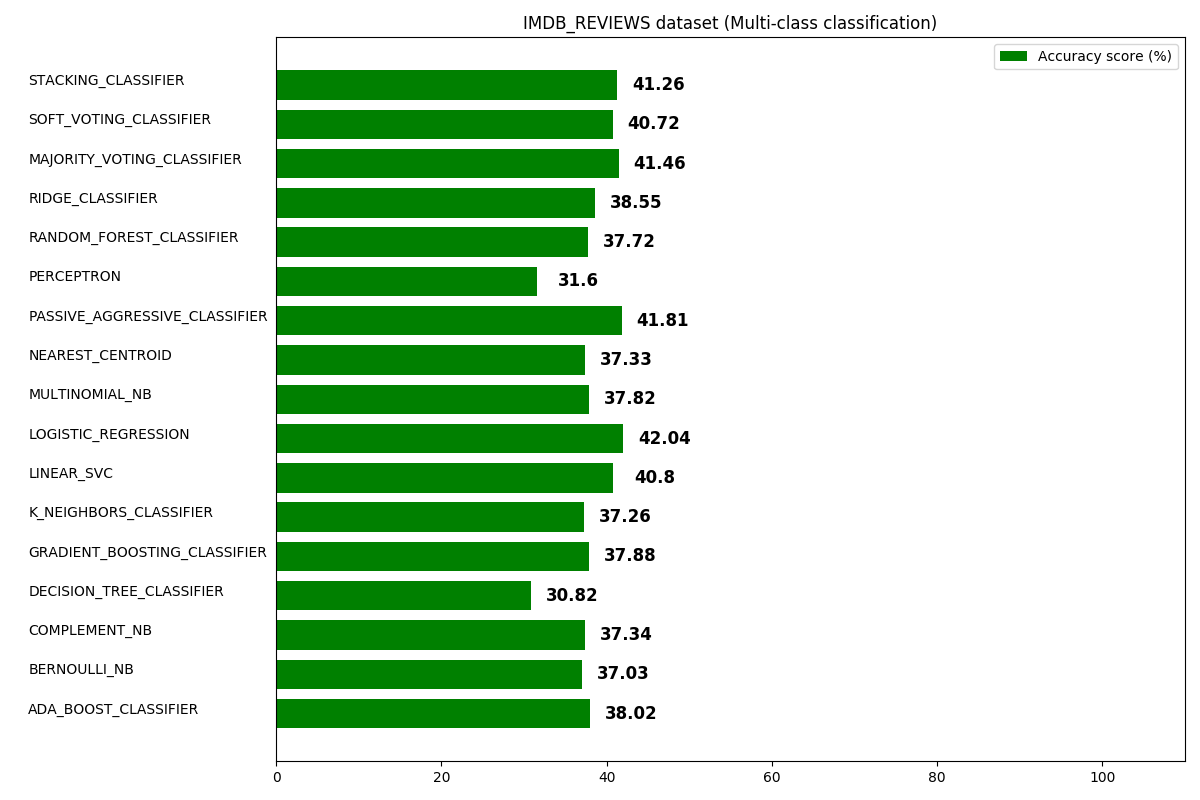
\includegraphics[scale = 0.21]{figs/all_classifiers_just_imdb_using_multi_class_classification/IMDB_REVIEWS_multi_class_classification-just_accuracy_score.png}
\caption{Accuracy score of the classifiers in the IMDB REVIEWS multi-class classification task using the best parameters}
\label{fig:imdb_multi_plot}
\end{figure}

For the deep learning models, we decided to use the following methodology: In each task, we trained both models for 20 epochs and recorded the evolution of the accuracy and loss on the training and validation sets. Figures \ref{fig:dl_imdb_kerasbinary}, \ref{fig:dl_imdb_multikeras} and \ref{fig:dl_20newskeras} show plots of that data for the \textbf{KERAS DL 1} model.

Looking at the validation set accuracy we observe that, as expected, the model improves for some epochs and then starts to get worse, because of overfitting. In each case, we obtained the number of epochs in which the model performance was best and then trained the model again for that amount of epochs. The results are summarized in Tables \ref{tab:deeplearningDL1} and \ref{tab:deeplearningDL2}.

Finally, we observe that the best performance in all three tasks was obtained by the KERAS DL 1 algorithm. Despite having a simple deep learning architecture compared to KERAS DL 2, it was able to outperform the other algorithms. Table \ref{tab:best_results} summarizes KERAS DL 1 test accuracy (best classifier) on each dataset.

\begin{table}[H]
  \caption{Deep learning Models with Keras DL 1}
  \label{tab:deeplearningDL1}
  \begin{tabular}{|p{2cm}|p{1cm}|p{2cm}|p{2cm}|}

\hline
 Dataset& Best epochs &
 Accuracy(\%) (Best epochs) & Accuracy(\%)(20 epochs) \\
 \hline
  20NEWS             & 10                    & 96.69                          & 96.66               
 \\
 \hline 
IMDB (binary)      & 1                     & 88.36                          & 83.23                        
\\
\hline 
IMDB (m-class) & 2                     & 89.10                          & 86.61   \\

\hline
    
  \end{tabular}
\end{table}

\begin{table}[H]
  \caption{Deep learning Models with Keras DL 2}
  \label{tab:deeplearningDL2}
  \begin{tabular}{|p{2cm}|p{1cm}|p{2cm}|p{2cm}|}

\hline
 Dataset& Best epochs &
 Accuracy(\%) (Best epochs) & Accuracy(\%)(20 epochs) \\
 \hline
  20NEWS             & 15                    & 96.08                           & 95.98               
 \\
 \hline 
IMDB (binary)      & 3                     & 86.33                          & 83.98                        
\\
\hline 
IMDB (m-class) & 2                     &  89.07                        & 86.15    \\

\hline
    
  \end{tabular}
\end{table}

\begin{table}[H]
  \caption{Test accuracy for the KERAS DL 1 model and Teacher Assistant (TA) baseline test accuracy in each task}
  \label{tab:best_results}
  \begin{center}
  \begin{tabular}{|c|c|c|}
    \hline
    Dataset & Test accuracy & TA Baseline test accuracy \\
    \hline
    20 NEWS (multi-class) & 96.69\% & 69.10\% \\
    \hline
    IMDB (binary)         & 88.36\% & 89.70\% \\
    \hline
    IMDB (multi-class)    & 89.10\% & ---     \\
    \hline
  \end{tabular}
  \end{center}
\end{table}

\section{Discussion and Conclusion}
\label{section:discussion}

During this project, we learned the usage of machine learning and deep learning for different datasets. We learned the impact of feature extraction in the accuracy of the algorithms such as removing stop words, feature extraction. By using the grid search, we were able to select the best parameters for all machine learning models, improving the accuracy score.

Future directions include trying more parameters in the grid search of all machine learning algorithms, explore our developed feature selection approach (chi-squared metric) to select the best features. Deep learning provided the best results, therefore future work also includes trying different deep learning architecture using more hidden layers or more neurons, use different activation functions, add new features and tune deep learning hyper-parameters.

\begin{figure}[H]
\centering
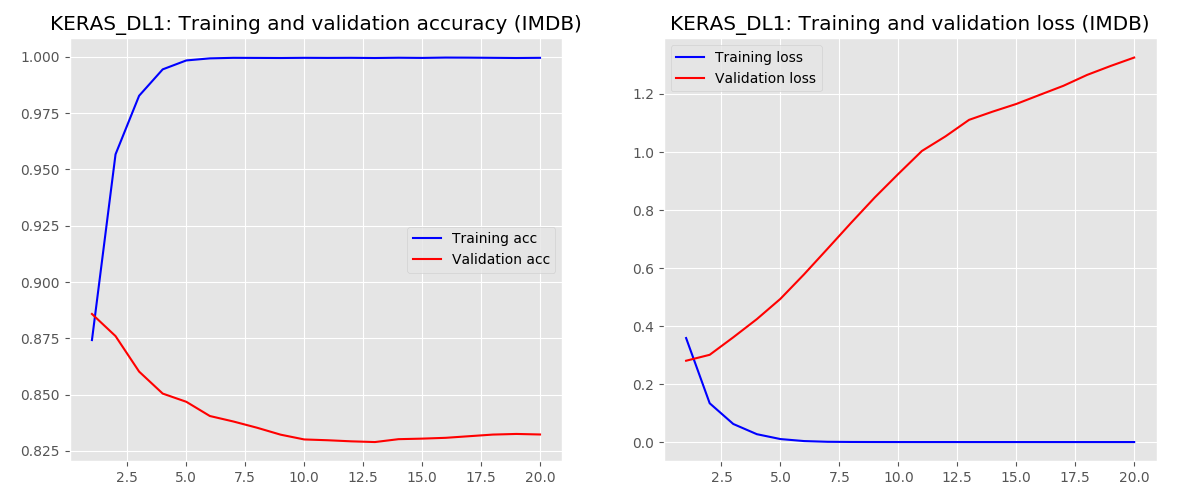
\includegraphics[scale = 0.22]{figs/deep_learning_using_keras/results_20newsgroups_and_imdb_using_binary_classification/20_epochs/KERAS_DL1_IMDB_REVIEWS_training_and_validation_accuracy_and_Loss.png}
\caption[Loss function of the deep learning model over the number of epochs for the binary classification on the IMDB Dataset]{Loss function of the deep learning model over the number of epochs for the binary classification on the IMDB Dataset}
\label{fig:dl_imdb_kerasbinary}
\end{figure}

\begin{figure}[H]

\centering
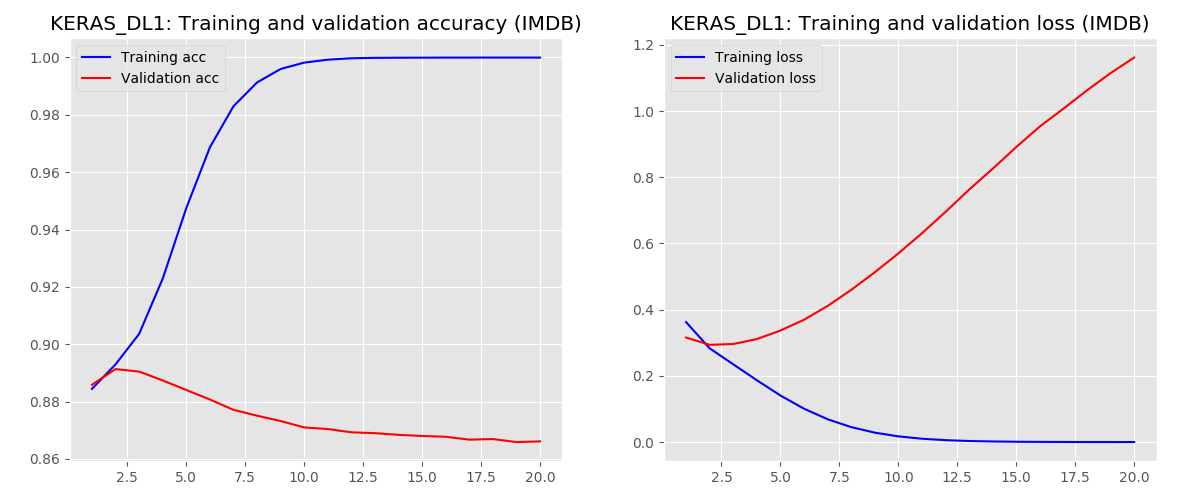
\includegraphics[scale = 0.22]{figs/deep_learning_using_keras/results_imdb_using_multi_class_classification/20_epochs/KERAS_DL1_IMDB_REVIEWS_training_and_validation_accuracy_and_Loss.png}
\caption[Loss function of the deep learning model over the number of epochs for the multi-class classification on the IMDB Dataset]{Loss function of the deep learning model over the number of epochs for the multi-class classification on the IMDB Dataset}
\label{fig:dl_imdb_multikeras}
\end{figure}

\begin{figure}[H]
\centering
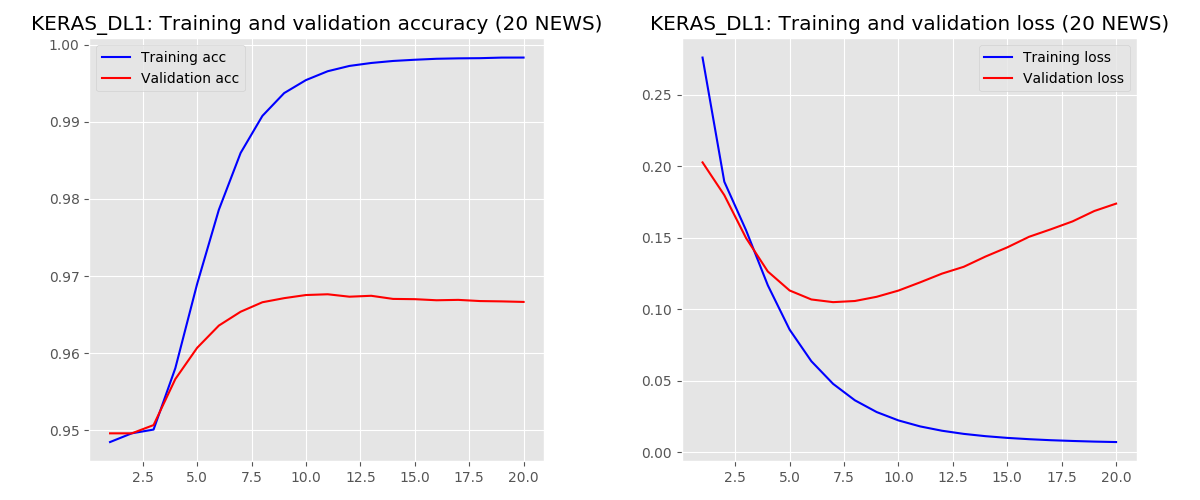
\includegraphics[scale = 0.22]{figs/deep_learning_using_keras/results_20newsgroups_and_imdb_using_binary_classification/20_epochs/KERAS_DL1_TWENTY_NEWS_GROUPS_training_and_validation_accuracy_and_Loss.png}
\caption[Loss function of the deep learning model over the number of epochs for the multi-class classification on the 20NEWSGROUP Dataset]{Loss function of the deep learning model over the number of epochs for the multi-class classification on the 20NEWSGROUP Dataset}
\label{fig:dl_20newskeras}
\end{figure}

\section{Statement of Contributions}
\label{section:contributions}

Ramon worked in the report and did all the code implementation (command-line interface (\textbf{extra}), datasets reading: 20 NEWS GROUPS multi-class, IMDB REVIEWS binary, IMDB REVIEWS multi-class (\textbf{extra}), data pre-processing using Scikit-Learn (stop words, strip accents, analyzer, binary parameters) and Natural Language Toolkit (NLTK)\footnote{NLTK: https://www.nltk.org/} applied in the KERAS DL 2, feature extraction, select some number of features using a chi-squared test (\textbf{extra}), cross-validation, grid search and save the best parameter in JSON used by the machine learning algorithms (\textbf{extra}), run the machine learning with the default and best parameters (\textbf{extra}), more metrics beyond accuracy score: precision score, recall score, f1 score, f beta score, jaccard score (\textbf{extra}), generated the result folder with .md files with images and tables (\textbf{extra}), created plottings: bar plot, training, and validation accuracy and loss (\textbf{extra}), developed all the five required machine learning classifiers and twelve more machine learning implementations including the voting classifier (majority and soft voting) and the stacking classifier (\textbf{extra}). Ramon also developed the second Keras deep learning model, KERAS DL 2 (\textbf{extra}), and fixed the first Keras deep learning model (KERAS DL 1)). Rafael developed the first Keras deep learning model KERAS DL 1 (\textbf{extra}) and worked on the report. Ege worked on the report.

\medskip

\small

\bibliography{bibliography}


\bibliographystyle{ieeetr}

\end{document}
